\documentclass[11pt,letterpaper]{article}

%%%%%%%%%%%%%%%%%%%%%%%%%%%%%%
\pagestyle{plain}                                                      %%
%%%%%%%%%% EXACT 1in MARGINS %%%%%%%                                   %%
\setlength{\textwidth}{6.5in}     %%                                   %%
\setlength{\oddsidemargin}{0in}   %% (It is recommended that you       %%
\setlength{\evensidemargin}{0in}  %%  not change these parameters,     %%
\setlength{\textheight}{9.0in}    %%  at the risk of having your       %%
\setlength{\topmargin}{0in}       %%  proposal dismissed on the basis  %%
\setlength{\headheight}{0in}      %%  of incorrect formatting!!!)      %%
\setlength{\headsep}{0in}         %%                                   %%
\setlength{\footskip}{.5in}       %%                                   %%

%%%%%%%%%%%%%%%%%%%%%%%%%%%%%%%%%%%%                                   

\usepackage[pdftex]{graphicx}
\usepackage{color}
\usepackage{url}
\usepackage{tabularx}
\usepackage{tikz}

% From PPoPP
\usepackage{amsmath}
\usepackage{amsfonts}
%\usepackage{graphicx}
%\usepackage{xspace}
\usepackage{verbatim}
%\usepackage{listings}
\usepackage{multirow}
\usepackage{subfigure}
\usepackage{pdfpages}
%% % Tweak spacing to fit in page limit if needed
%% % ============================================
%% % gap between text and figs/tables:
%% \addtolength\textfloatsep{-0.2in}
%% % gap between figs/tables and other figs/tables
%% \addtolength\floatsep{-0.1in}
%% % gap between figure and caption
%% \addtolength\abovecaptionskip{-0.05in}
%% \addtolength\intextsep{0in}

\hyphenation{ }

\setlength{\parindent}{0.5cm}

\newif\ifdraft
% comment out the next line to turn off comments
%\drafttrue

\ifdraft
  \definecolor{darkgreen}{rgb}{0,0.5,0}
  \newcommand{\manish}[1]{ {\it \color{red} \{#1 -Manish}}}
  \newcommand{\hasan}[1]{ {\textcolor{blue} { #1 -Hasan }}}
  \definecolor{orange}{rgb}{0.7,0.5,0.0}
  \newcommand{\klasky}[1]{{\textcolor{orange}{ #1 -Scott }}}
  % Red star denotes items that need further work or discussion
  \newcommand{\TODO}[1]{{\textcolor{red}{ TO DO: #1 }}}
\else
  \newcommand{\klasky}[1]{}
  \newcommand{\hasan}[1]{}
\fi

%\newcommand{\ititle}{\textsc{\textbf{HESK}}}
\newcommand{\ititle}{\textsc{HESK}}
\newcommand{\insitu}{\textit{in situ }}

\let\oldenumerate\enumerate
\renewcommand{\enumerate}{
      \oldenumerate
      \setlength{\itemsep}{1pt}
      \setlength{\parskip}{0pt}
      \setlength{\parsep}{0pt}
}

% A definition we do not want the reader to forget
\newcommand{\defn}[1] {\textbf{\textit{#1}}}

\definecolor{teal}{rgb}{0.06,0.3,0.3}
\definecolor{maroon}{rgb}{0.5,0.0,0.25}
\definecolor{darkblue}{rgb}{0.0,0.2,0.75}
\definecolor{darkred}{rgb}{0.7,0.0,0.0}
\definecolor{darkgreen2}{rgb}{0,0.35,0}

\newcommand*\circled[1]{\tikz[baseline=(char.base)]{
  \node[shape=circle,draw,inner sep=2pt] (char) {#1};}}


\begin{document}
\begin{comment}
\noindent
\textbf{Pre-proposal Cover Sheet}
\newline
\vskip .1in
Storage Systems and Input/Output for Extreme Scale Science 
Scale 2 (LAB 14-1043)

\vskip .3in

\noindent
\textbf{Project title:}
\vskip .1in
Hierarchal Extreme Scale Knowledge Management


\vskip .3in

\noindent
\textbf{Principal investigator:}
\vskip .1in

Scott Klasky klasky@ornl.gov

\vskip .2in

\noindent
\textbf{Co-principal investigator:}
\vskip .1in

Manish Parashar, Rutgers, parashar@rutgers.edu, 732-445-5388
Carlson Malzahn, UCSC
Jay Lofstead, Sandia, gflofst@sandia.gov, 505-284-5803


\vskip .2in

\noindent
\textbf{Senior Personnel:}
\vskip .1in
Hasan Abbasi, ORNL
Mark Ainsworth, ORNL
Matthew Curry, Sandia
Qing Liu, ORNL
Lee Ward, Sandia



\begin{tabular}{| l| r| r| r| r| }
\hline
  \emph{Institution} & \emph{Year 1} & \emph{Year 2} & \emph{Year 3} \\
\hline
Oak Ridge National Laboratory & \$350,000 & \$350,000 & \$350,000	\\
\hline
  Rutgers University & \$175,000 & \$175,000 & \$175,000 \\
\hline
  University of California Santa Cruz & \$160,000 & \$160,000 & \$160,000 \\
\hline
  Sandia National Laboratories & \$360,000 & \$360,000 & \$360,000 \\
\hline
  Total & \$1,250,000 & \$1,250,000 & \$1,250,000 \\
\hline
\end{tabular}
\newpage

\end{comment}
%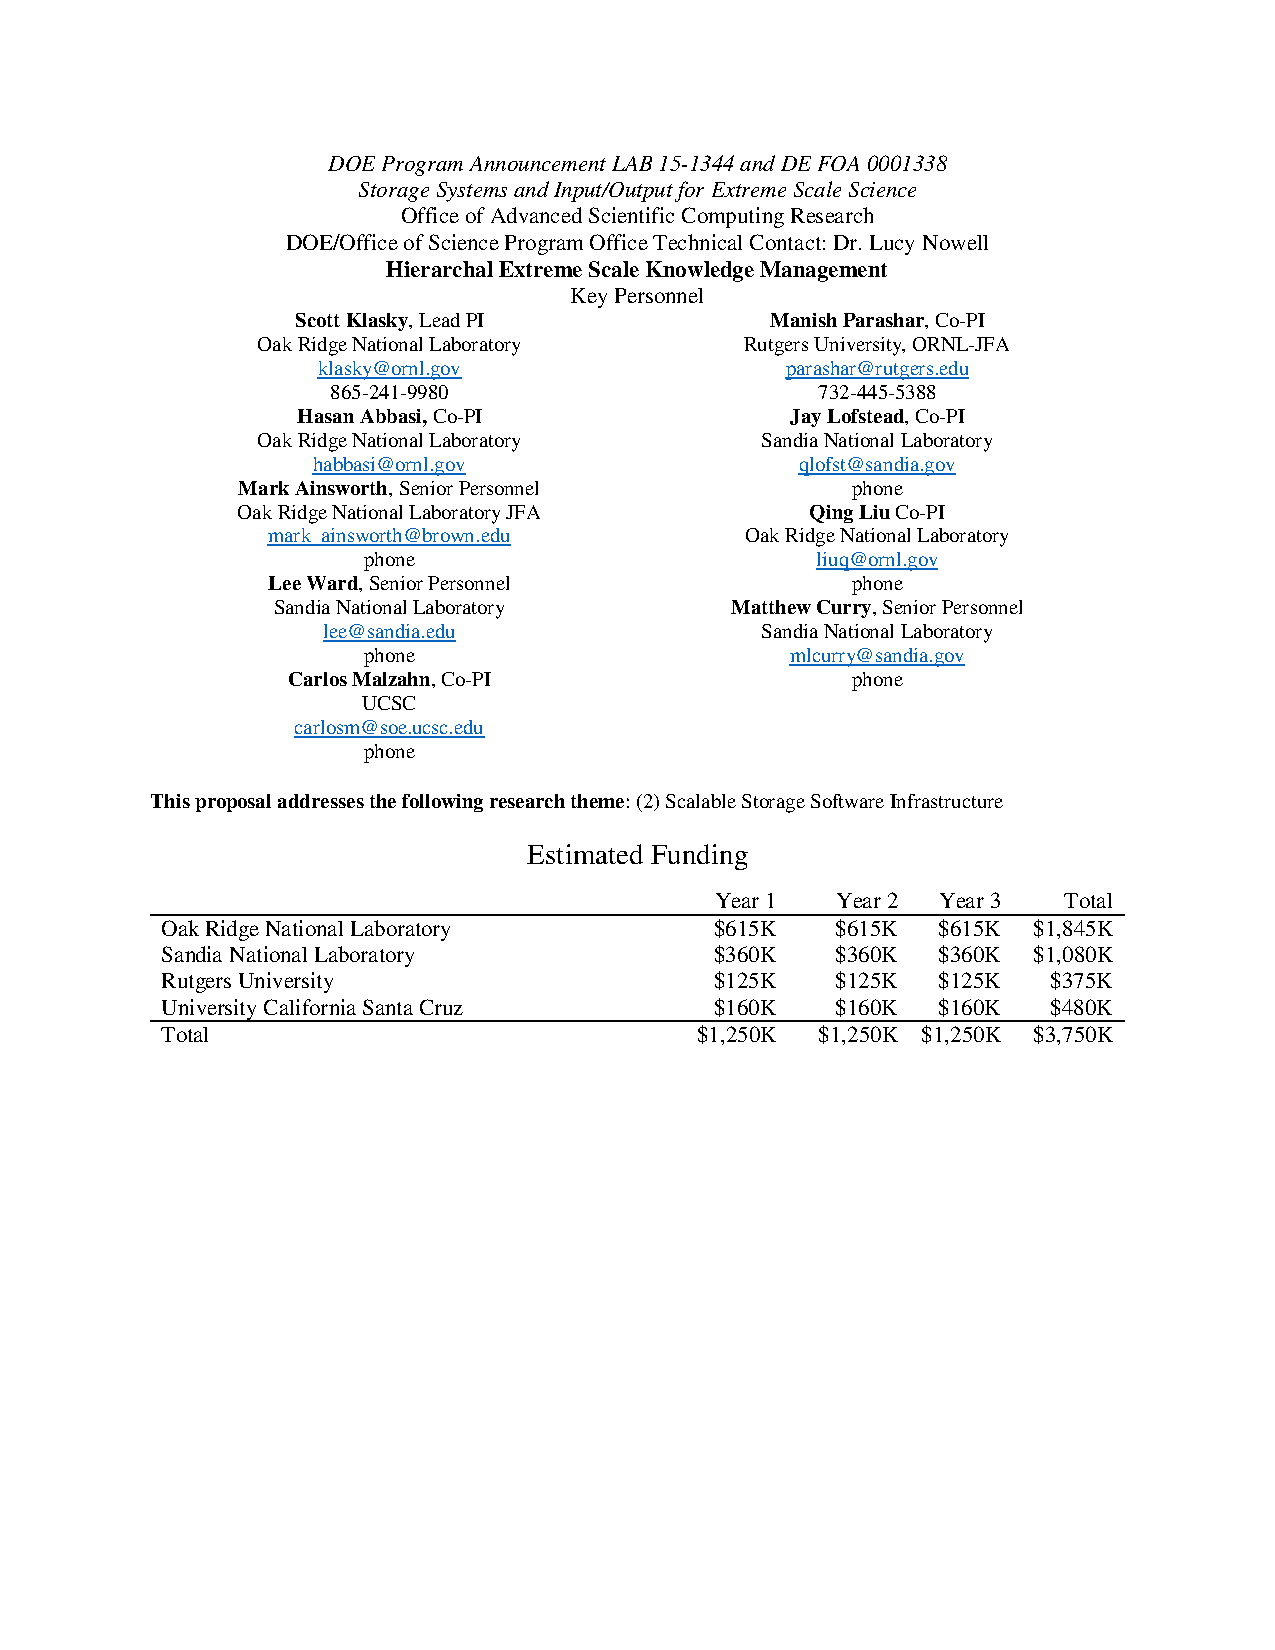
\includepdf[pages={1}]{ornl-cover.pdf}
%\pagebreak

\author{
  \IEEEauthorblockN {
    PI: Scott Klasky, % \IEEEauthorrefmark{1},
    Co-PI Manish Parashar % \IEEEauthorrefmark{1}
  }
  \IEEEauthorblockA {
    % \IEEEauthorrefmark{1}
    Mathematics and Computer Science Division,
    Argonne National Laboratory,
    Argonne, IL, USA}
}

%\maketitle

% Heilmeyer Points: from http://www.csee.umbc.edu/~finin/home/heilmeyerCatechism.html
% 
% \begin{enumerate}

% \item What is the problem, why is it hard? 

% \item How is it solved today?
%  Fig A: much 

% \item What is the new technical idea; why can we succeed now?
%  Integration of proven components into an architecture that solves
%  problems. New research will resolve remaining technical hurdles.

% \item What is the impact if successful?
%  Users and developers will be able to ...

% \item How will the program be organized?
%  Participants and focus areas

% \item How will intermediate results be generated?
%  Toolkit snapshots and application

% \item How will you measure progress?
%  Provide metrics

% \item What will it cost?
%  Cover sheet

% \end{enumerate}
%

{\bf Title of Pre-application:} Hierarchal Extreme Scale Knowledge Management \par
{\bf Principal Investigator:} Scott Klasky, Group Leader, ORNL, 854-241-9980, klasky@ornl.gov \par
{\bf Funding Opportunity Announcement Number: DE-FOA-0001338} \par
{\bf List of all co-PIs and Key/Senior Personnel} \par
Hasan Abbasi, Oak Ridge National Laboratory \par
Mark Ainsworth, Oak Ridge National Laboratory JFA, Brown University \par
Matthew Curry, Sandia National Laboratory\par
Qing Gary Liu, Oak Ridge National Laboratory \par
Jay Lofstead, Sandia National Laboratory \par
Kimmy Mu, Oak Ridge National Laboratory \par
Carlos Malzahn, U. Cal. Santa Cruz \par
Manish Parashar, Rutgers University, Oak Ridge National Laboratory \par
Sudharshan Vazhkudai, Oak Ridge National Laboratory \par
Lee Ward, Sandia National Laboratory \par
\vskip 0.2 in



\underline{\textbf{Objectives:}}
Exascale scientific discovery will be severely bottlenecked without sufficient
new research into managing and storing the large amounts of data that will be
produced during the simulation, and analyzed for months afterwards.  Our goal
in this project is to address associated I/O and storage challenges in the context 
of current and emerging storage landscapes, and expedite insights into mission 
critical scientific processes. To that end, we will build on the capabilities offered
by ADIOS and DataSpaces that provide I/O abstractions and services, the Sirocco 
peer-to-peer file system under development at Sandia and the object storage 
and annotation expertise of UC Santa Cruz, to develop a application and 
multi-tier storage aware data management solution. Our solutions will provide
novel functionalities and APIs for 
% It will center upon a multi-tier storage-aware approach and incorporate new
%functionalities, extended object metadata and APIs for 
1) specifying, at the application level, data annotations than enable the qualification
 of the relative importance and utility of data objects, and enable them to be 
 mapped at runtime to appropriate storage capabilities across the storage hierarchy;
2) specifying selectable performance/quality/cost tradeoffs from both application and system perspectives; and
3) evaluating and executing these tradeoffs at runtime, in an autonomic manner,
during data placement and movement, using techniques such as application-aware 
data compression (both lossy with specified error bounds and lossless), re-computation, 
reader prioritization, etc.
%2) a selectable performance/quality tradeoff when reading data, and
%the ability to recompute data if needed, and
%3) incorporate reader prioritization for data annotation, placement, and data
%quality when writing data.  
The key challenge in this project is defining and maintaining the metadata
 connecting different object quality and utility levels, and using this metadata 
 to most appropriate manage the placement and access of data object based on 
 user/application intent/contraints and storage system state.
% to best enabling the user with the best possible outcomes 
 %given the user intent and the storage system state. 
The new user APIs required to interact with this rich metadata system will drive effective
use of the entire middleware and storage stack. 
The project is comprised of a team with strong expertise in I/O middleware (ORNL, Rutgers), file system (SNL,
UCSC) and storage (UCSC), and connect and coordinate these key storage
components in a seamless fashion.

\manish{I believe this analogy needs to be developed further -- the point we are trying to make here, i.e., autonomic cross layer management, negotiation, are not completely obvious.}
Our approach can most easily be understood by considering a road navigation
program. Similar to the navigation program, we will offer a coarse grained,
fast overview of a data set with progressively more detail in areas of interest
such as those contain features, and less detail in areas without. These progressively
more detailed data views require more storage space and time to retrieve. By
incorporating middleware informed of either the criteria for identifying areas of interest
or the intended use locations, it will be able to selectively store
data at different quality levels, with bounded errors in the case of lossy
compression, and allow a user to select what data to retrieve by specifying
both an acceptable retrieval timeframe and error bound. 
%If the request
%cannot be fulfilled, the storage system can negotiate with the user providing
%information about the quality and timeframes available for a subsequent
%request.
%%%%%%%%%%%% I am not sure if we should do this type of expert system in the project.
The user may also specify guidelines that are funneled through the I/O middleware and 
provide advice on how to react if the timeframe and error bound cannot be accepted.

Our objective here is to reduce the time to knowledge, an end-to-end metric
relevant to the scientific discovery process. We will explore beyond the traditional high
volume I/O pattern of checkpoint/restart, and will address the challenges posed
by other essential data access patterns in the knowledge gathering process.
Through a deeper insight into the scientific process we will encode and utilize
accuracy and errors as optimization parameters. 
For example, scientific simulations contain approximations, as do measurements
from observations and experiments, and depending on the goal, these
approximations are acceptable. We can leverage this observation to optimize the
presentation of data to the user and to implement various tradeoffs  -- users can 
ask for information within a given accuracy bound, allowing
us to offer a mode for re-computation vs. data storage and retrieval.

%
{\bf: please list other things from OLCF}.
%


\underline{\textbf{Key Technical Approach:}}
Our overall technical approach is based on an application-aware runtime
realization of tradeoffs in data representation, data placement and data
access. We will allow users to be able to ``plug-in'' their knowledge 
about the data, not as bytes but as motifs, thus allowing the I/O and 
storage system to understand user
intentions and the relationships between data objects, as well as data access
and transport patterns. This will facilitate efficient mapping of data from
user space onto various storage tiers, and application-guided
data reductions.

The I/O and storage system produced from the project will
enable highly flexible data access modes that are common in data analytics. 
\textbf{First}, data re-computation is allowed to re-generate
data with higher accuracy, if the associated computing and I/O cost is lower
than retrieving the target data from a ``slow'' tier. 
\textbf{Second}, exploratory analysis
operations frequently entail an overall data set view followed by targeted data
exploration on extracted features. 
In particular, the ``overview'' access mode gives a quick but approximate
data view that can guide feature selection offering rapid coarse-grained data
exploration without requiring loading the high-accuracy data from
storage. Based on the granularity requested, the accuracy and size of the data
returned can be adjusted. In the most extreme setting, the original data can
be retrieved at the time cost of moving the potentially huge data quantity.
\textbf{Third}, to ensure available storage for subsequent operations, we will
offer automatic data migration based on user annotations for required data
lifetimes using monitoring and learning techniques. Unlike existing approaches,
this will be tempered both by the user annotations and through learned access
patterns.  While past access patterns may not indicate future access because
the simulation run purpose may have changed, we are focused on scalability
where runs are subsequently larger as the simulation prepares for a capability
run.  By learning from the output and access patterns during this run sequence,
we can accurate decide how to place and organize data for the critical
capability runs. 
\textbf{Fourth}, we anticipate storing multiple data copies, each
compressed in different ways according to the underlying media, some of these
copies will disappear based on storage pressures, but data persistence will be
maintained according to user specifications. Assuming a relatively low latency
cache layer before a tape system, we can offer exploratory data access
reserving pulling data from tape to just the data required. This will save
scientists time and make data stored on tape usable without long delays.

Our research efforts will be heavily focused on the need to, in a coordinated
manner, adapt data and metadata retention policies to the dynamic resource
balancing that will need to take place between the application, OS/R, and
hardware.

The success of this project will  provide insights into how to build autonomic
middleware and storage layers which can interact well with each other, and take
user-provided hints. Today, data is reduced by application scientist who have
limited information on what the storage layer can provide. They often make
compromises based on this limited knowledge and either tune their output for
writing or reading performance. This data then gets moved to other locations,
and much of the tuning is lost when the data is read back during their post
processing. Furthermore, there is a limited set of operations which users will
be able to stage to other staging nodes for real-time-reduction and
visualization. 


%\includepdf[pages={1}]{COI.pdf}

\end{document}

%%% End: 
